\documentclass[12pt]{article}

% This first part of the file is called the PREAMBLE. It includes
% customizations and command definitions. The preamble is everything
% between \documentclass and \begin{document}.

\usepackage[margin=1in]{geometry}  % set the margins to 1in on all sides
\usepackage{graphicx}              % to include figures
\usepackage{amsmath}               % great math stuff
\usepackage{amsfonts}              % for blackboard bold, etc
\usepackage{amsthm}                % better theorem environments
\usepackage{amssymb} 
\usepackage{mathptmx}
\usepackage{graphicx}
\usepackage{enumerate}
\usepackage{listings}
\usepackage{xcolor}
\usepackage{array}

% various theorems, numbered by section

\newtheorem{thm}{Theorem}[section]
\newtheorem{lem}[thm]{Lemma}
\newtheorem{prop}[thm]{Proposition}
\newtheorem{cor}[thm]{Corollary}
\newtheorem{conj}[thm]{Conjecture}
\newtheorem{mydef}[thm]{Definition}


\lstset{
	basicstyle          =   \sffamily,          
	keywordstyle        =   \bfseries,          
	commentstyle        =   \rmfamily\itshape,  
	stringstyle         =   \ttfamily,  
	flexiblecolumns,                
	numbers             =   left,   
	showspaces          =   false,  
	numberstyle         =   \fontsize{5}{skip},    
	showstringspaces    =   false,
	captionpos          =   t,      
	frame               =   lrtb,   
}

\lstdefinestyle{cpp}{
	language        =   cpp, 
	basicstyle      =   \fontsize{5}{skip},
	numberstyle     =   \fontsize{5}{skip},
	keywordstyle    =   \color{blue},
	keywordstyle    =   [2] \color{teal},
	stringstyle     =   \color{magenta},
	commentstyle    =   \color{red}\ttfamily,
	breaklines      =   true,   
	columns         =   fixed,  
	basewidth       =   0.5em,
}
\begin{document}


\title{ CSE 102 Spring 2021\\
	Advanced Homework Assignment 6}

\author{Jaden Liu \\ 
University of California at Santa Cruz\\
Santa Cruz, CA 95064 USA }

\maketitle


\section{AdvHW6} 
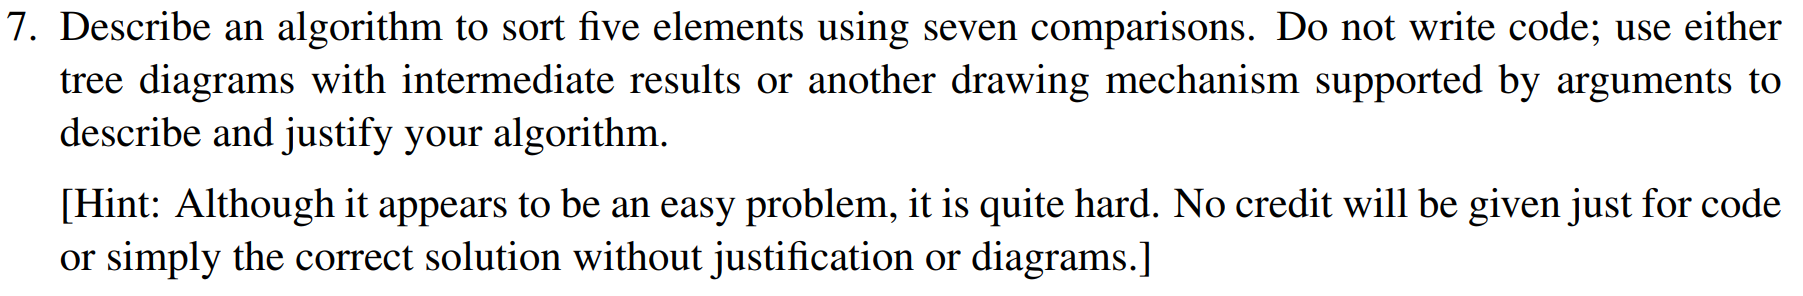
\includegraphics[scale=0.25]{adv_7.png}
Assume we have the array A[] = \{a,b,c,d,e\}.
\begin{proof}[Algorithm]
	Assume we need to sort the array descending order. The graph below has shown the worst occasion.\\
		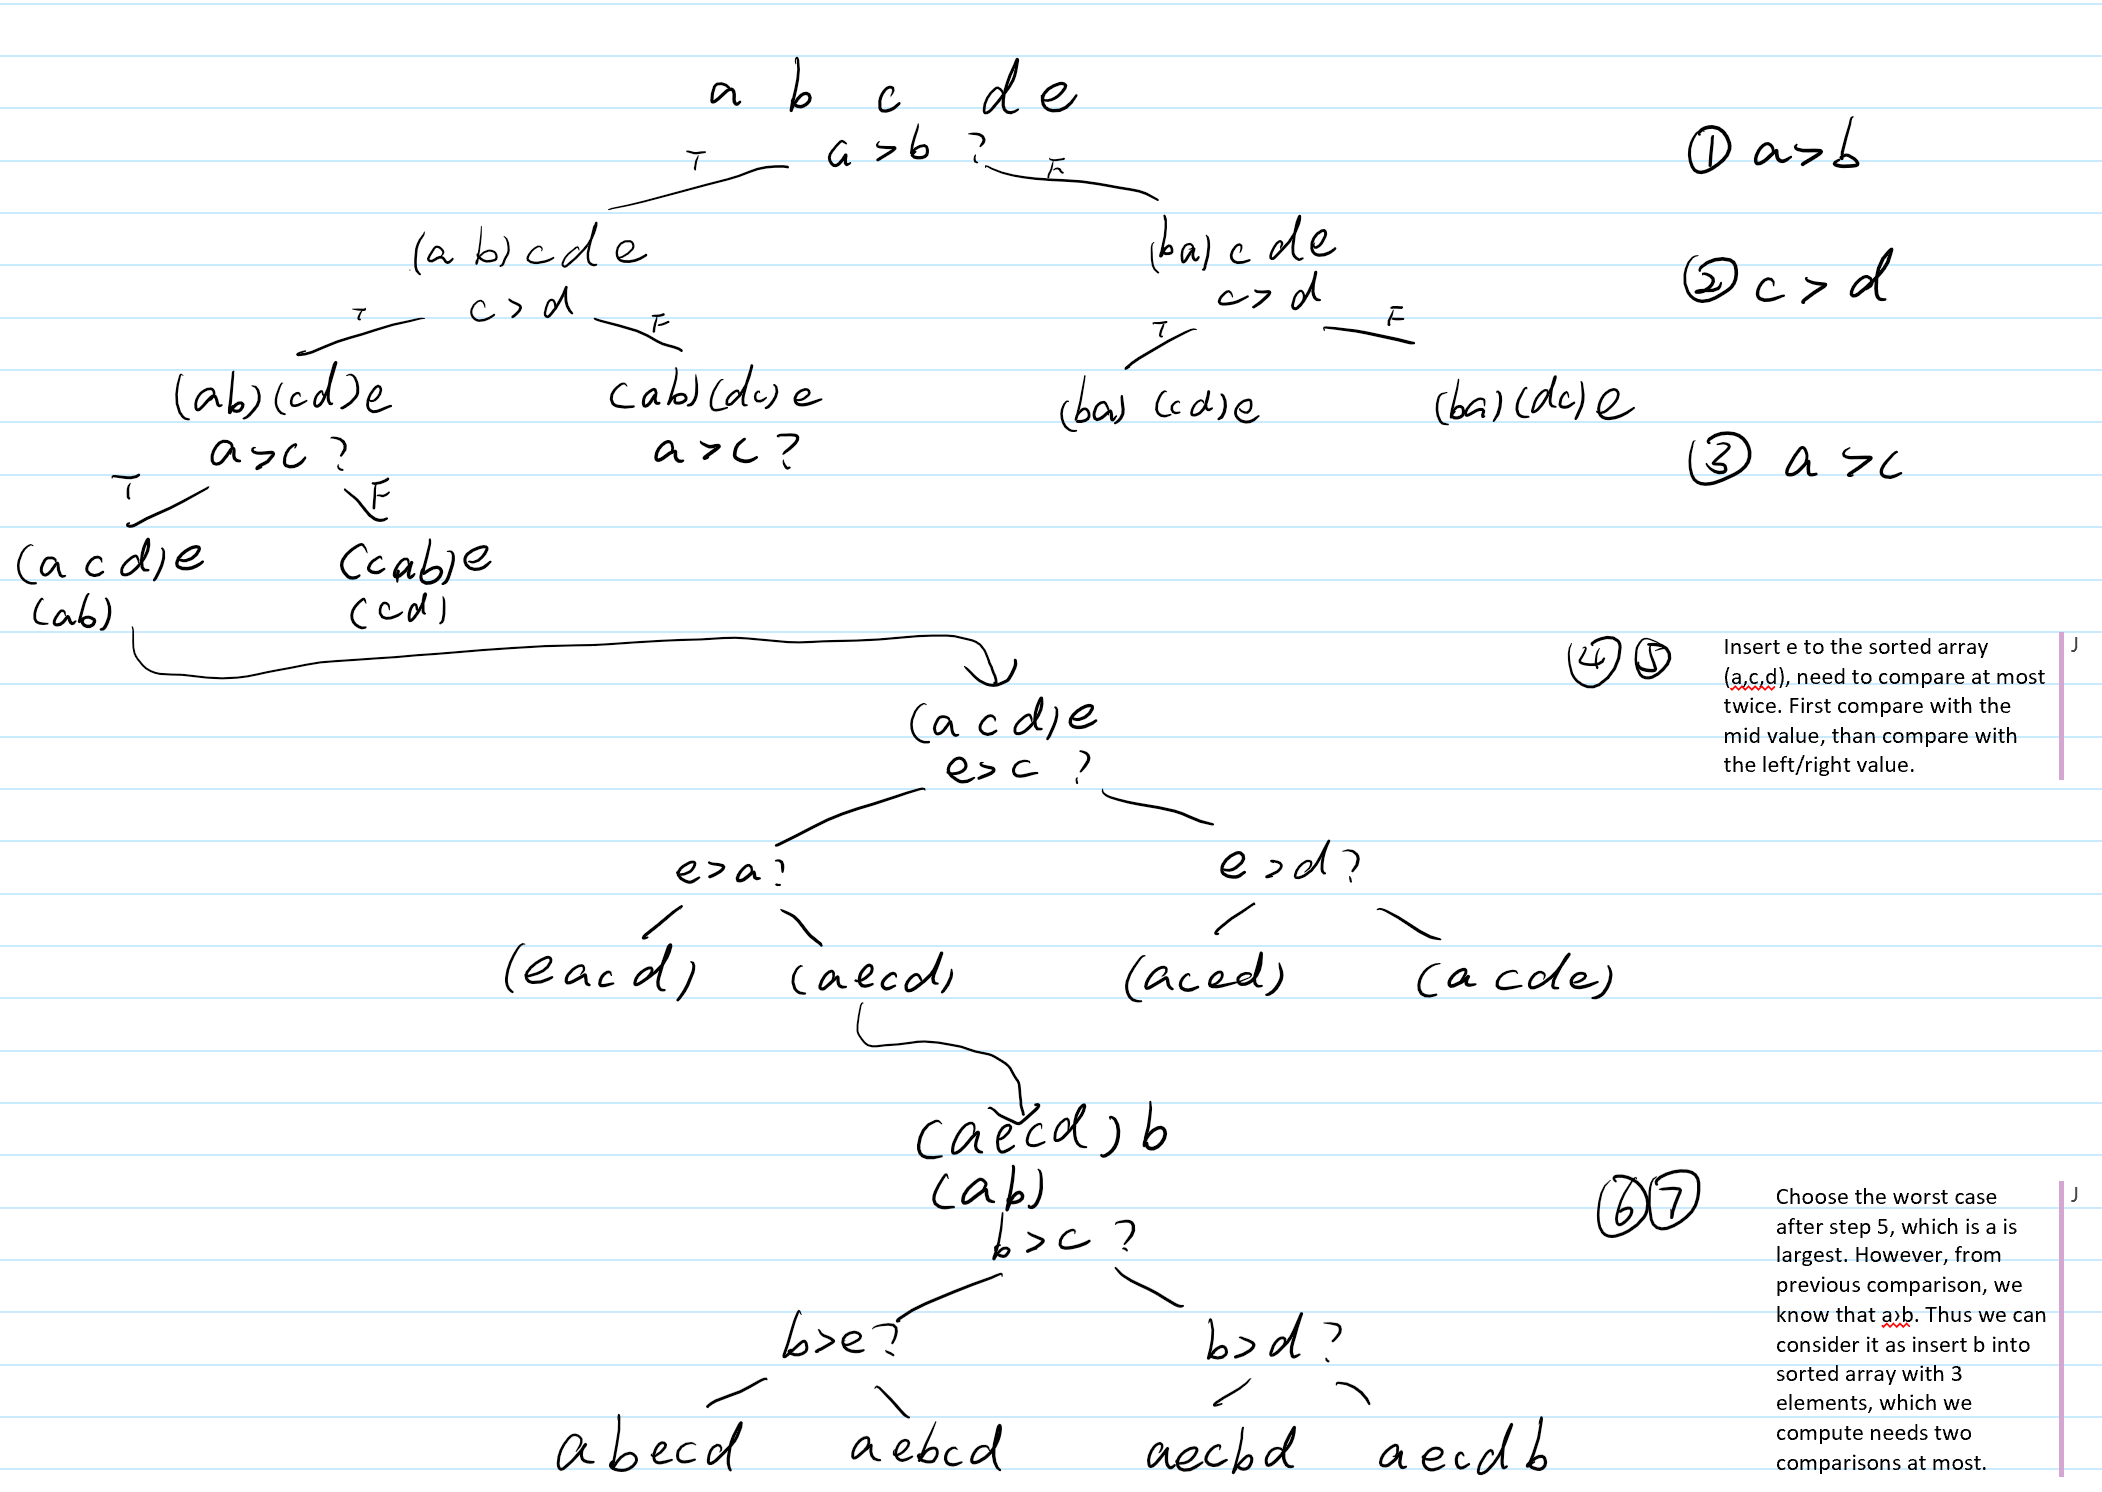
\includegraphics[scale=0.25]{adv_1.png}
		
	1\&2. Compare $a$ with $b$; compare $c$ with $d$. Then we get $(a,b)(c,d)e$. We use parenthesis to mean that the array has been sorted. total\_com=1+1=2\\
	
	3. Compare the two sorted array's first element, then we get two branches. If $a>c$, then we get the sorted array $(a,c,d)$; otherwise we get the sorted array $(c,a,b)$. total\_com=2+1=3\\
	
	4\&5. We need to insert $e$ into the three element sorted array $(a,c,d)$ or $(c,a,b)$, which takes at most 2 comparisons.(first compare with mid value, then compare with the left/right value) total\_com=3+2=5\\
	
	6\&7. Now we have a 4 element sorted array and single element $b$ with a relation $a>b$, thus, $b$ has to appear after $a$. The worst case is that $a$ is the largest element in the sorted array. In this case, it's like the case inserting $b$ into a three elements sorted array(the three elements that are smaller than $a$), which takes up to 2 comparisons. total\_com=5+2=7\\
\end{proof}
\begin{proof}
	In this problem, we have $5!=120$ different permutations that can be performed. After each comparison, we have two branches, hence we need at least $\log_2{5!}=6.907 \approx7$ times branch to hold such an amount of permutations. i.e. the lower bound of the problem is 7 times comparisons.\\ 
\end{proof}
\begin{proof}[Thought to found this solution]
	Here is the thought how we can get this solution:
	
	1. At first it's hard to think of the correct way, we have to use lower bounds to eliminate the inpossible ways to approach our answer. Initially we have $2^7=128$ possible answer and $5!=120$ different permutations.
	
	2. The first compare is the equally good for any of the two element comparison; for convenience, just compare $a$ and $b$, then we eliminate permuatation to 3*4*5=60, and we still have $2^6=64$ possible answers, good.
	
	3. Compare element c with either element in the first comparison or with other element that are not in the first comparison. With first comparsion: permutation = 4*5+4*5=40, which is out of $2^6=32$ possible answers. With other element: permutation = 5*6=30, which is still under constraints.
	
	4. Compare element e with either first or second comparing elements or compare the two sorted array? Compare e: permutation = (4+3+2+1) * 2 = $20 > 2^4=16$. Compare two sorted array: permutation = 3*5=15, still under constraints.
	
	5. Compare either e with three sorted array or the previous 2 sorted array. 3: permutation = 2*2=4. 2: permutation = 6*2 =12. So we have to compare e with the sorted 3-element array. 
	
	6.Now it is easier to think of the correct answer without using the lower bounds to restrict the answer. We can get the final answer by normal thinking.
\end{proof}



\end{document}
